\documentclass{article}
\usepackage{booktabs}
\usepackage{caption}
\usepackage{subcaption}
\usepackage[T1]{fontenc}
\usepackage[british]{babel}
\usepackage{microtype}
\usepackage{fontspec}
\usepackage{xcolor}
\usepackage{xurl}
\usepackage{pdfpages}
\usepackage{enumitem}
\usepackage{lineno}
\usepackage{float}
\usepackage{natbib}
\usepackage{longtable}
\usepackage{geometry}
\usepackage{tabularx}
\setmainfont[Mapping=tex-text,Ligatures={Common,Rare,Discretionary}]{Linux Libertine}
% Define colors
\definecolor{blue}{RGB}{33,150,209}
\definecolor{red}{RGB}{255,0,0}

% Set geometry for the page
\geometry{a4paper, margin=1in}

% Line numbers settings
%\setlength{\linenumbersep}{5pt}
%\linenumbers

% Modify URL and texttt fonts
\renewcommand{\UrlFont}{\ttfamily\small}
\let\oldtexttt\texttt
\renewcommand{\texttt}[1]{{\ttfamily\small\nolinkurl{#1}}}

% Custom box command for drafting purposes
\usepackage{tcolorbox}
\newcommand{\cbox}[1]{
    \begin{tcolorbox}[hbox, colback=red!5!white, colframe=red!65!black, boxrule=0.25pt, boxsep=2pt, left=2pt, right=2pt, top=1pt, bottom=1pt]
        \small\sffamily #1
    \end{tcolorbox}
    }

\usepackage[colorlinks=true, allcolors=blue]{hyperref}
\begin{document}

\title{\textbf{Supplementary material for the T-reX Manuscript}}
\author{Stewart Charles McDowall, Elizabeth Lanphear, Stefano Cucurachi, Carlos Felipe Blanco  \\
    \textit{Institute of Environmental Sciences (CML), Leiden University, Leiden, The Netherlands}}
\date{1 December 2024}

\maketitle
\tableofcontents
\listoffigures
\listoftables
\clearpage


% \section*{Supplementary material}\label{sec:supplementary}
% The supplementary material contains the following:
% \begin{enumerate}
%     \item Metadata of the T-reX Python package
%     \item Details of the modules and user configuration
%     \item Description of the computational workflow
%     \item Modular flowchart of T-reX
%     \item Example of the terminal output of T-reX
%    \item{Python scripts used in the case study}
%     \item Complete tabulated results of the case study
%     \item Complete visualisations from the case study
% \end{enumerate}


\section{Metadata of T-reX}

\begin{table}[h]
    \caption{T-reX tool metadata}\label{tab:metadata}
    \centering
    \begin{tabular}{ll}
        \toprule
        \textbf{Item}     & \textbf{Details}                             \\
        \midrule
        Current version   & 0.1.21                                       \\
        DOI               & \url{zenodo.org/doi/10.5281/zenodo.10431180} \\
        Code repository   & \url{github.com/Stew-McD/T-reX}              \\
        License           & CC0--1.0 license                             \\
        Versioning system & git                                          \\
        Language          & Python                                       \\
        Documentation     & \url{T-reX.readthedocs.io}                   \\
        Main dependencies & \texttt{brightway, premise, wurst}           \\
        \bottomrule
    \end{tabular}
\end{table}

\section{List of modules in the T-reX Python package}

\subsection{Functional modules}
\begin{itemize}
    \item \texttt{future\_scenarios}: Creates prospective LCA databases based on future scenarios.
    \item \texttt{explode\_database}: Responsible for expanding a \texttt{brightway} database into detailed exchange lists.
    \item \texttt{search\_waste}: Provides functions for searching and categorising waste generation-related exchange data.
    \item \texttt{search\_material}: Provides functions for searching and categorising material demand-related exchange data.
    \item \texttt{make\_custom\_database}: Facilitates the creation of custom databases based on the waste and material search categories.
    \item \texttt{method\_editor}: Manages the custom LCIA methods for waste and material footprint calculations.
    \item \texttt{exchange\_editor}: Appends `pseudo-biosphere' exchanges to activities to match their waste generation and material demand exchanges in the technosphere.
    \item \texttt{verify\_database}: Performs verification of the manipulated databases.
\end{itemize}

\subsection{Configuration modules}
\begin{itemize}
    \item \texttt{custom\_config}: Provides functions for managing the configuration of the T-reX package.
    \item \texttt{user\_settings}: The main configuration file, for defining the project and database settings (user editable).
    \item \texttt{queries\_waste}: Defines search parameters and categories for waste generation exchanges (user editable).
    \item \texttt{queries\_materials}: Defines search parameters and categories for material demand exchanges (user editable).
\end{itemize}

\section{Description of the computational workflow}


\subsection{Generation of prospective LCA databases}

Future waste and material footprints can be projected using the \texttt{future\_scenarios} module, which uses \texttt{premise} to generate prospective scenario databases based on the configuration in \texttt{user\_settings}. These prospective databases can be custom-defined by the user or can be constructed with the future projections of the integrated assessment models such as IMAGE~\citep{stehfest2014image} and REMIND~\citep{remind2020model}, which offer a range of options aligned with the Shared Socioeconomic Pathways (SSPs)~\citep{ssp2020ghg} that can be paired with a variety of mitigation scenarios.

\subsection{Database expansion}
The \texttt{explode\_database} module uses \texttt{wurst} to deconstruct LCA databases into a list of individual exchanges representing all of material and energy flows in the technosphere model. This dataset being converted into a pandas DataFrame and stored as a binary \texttt{.pickle} file for subsequent analysis.

\subsection{Waste and material flow identification and categorisation}

The \texttt{search\_waste} and \texttt{search\_material} modules apply user-defined search parameters from \texttt{queries\_waste} and \texttt{queries\_materials} to identify relevant waste and material flows in the list of technosphere exchanges generated by \texttt{explode\_database} and categorises them accordingly. The results of the search functions are stored in \texttt{.csv} files for subsequent use in T-reX's workflow.

\subsubsection{Waste exchanges}\label{sec:method-T-reX-waste_exchanges}


The logic of screening for waste exchanges is based on a set of boolean search queries (`AND', `OR', and `NOT') that are applied in a list comprehension to the names of every exchange in the LCA database (see `search\_queries.py' for the full list). In this way, the search queries enable classification into categories (such as `hazardous solid' and `incineration liquid') and permit the identification of waste exchanges in addition to those directly connected to waste treatment processes. The search queries are tailored to the specific database and the user can easily modify them to suit their needs. In the default settings, there are a total of 18 waste classifications (9 categories, each separated into liquid and solid waste) For example, the identification of `non-hazardous solid' waste exchanges is based on the following search query; \texttt{AND = [`waste'], NOT = [`hazardous', `radioactive'], UNIT = [`kilogram']} (this can also be inferred and confirmed by comparison with the difference between the results of `total solid' and `hazardous solid').

The default waste categories and their search logic are listed in \autoref{tab:waste_categories}.

\begin{table}[ht]
    \centering
    \caption{Waste categories in the default configuration of T-reX}\label{tab:waste_categories}
    \begin{tabularx}{\textwidth}{p{2.5cm}p{1cm}p{1.5cm}XX}
        \toprule
        \textbf{Waste Category} & \textbf{AND} & \textbf{AND +} & \textbf{OR}                                      & \textbf{NOT}                   \\
        \midrule
        digestion               & waste        & digestion      &                                                  &                                \\
        composting              & waste        & composting     &                                                  &                                \\
        open burning            & waste        & burning        &                                                  &                                \\
        incineration            & waste        & incineration   &                                                  &                                \\
        recycling               & waste        & recycling      &                                                  &                                \\
        landfill                & waste        &                & landfill, dumped, deposit                        &                                \\
        hazardous               & waste        &                & hazardous, radioactive                           & non-hazardous, non-radioactive \\
        non-hazardous           & waste        &                &                                                  & hazardous, radioactive         \\
        carbon dioxide          & waste        &                & carbon dioxide storage, carbon dioxide, captured & methane                        \\
        total                   & waste        &                &                                                  &                                \\
        \bottomrule
    \end{tabularx}
\end{table}


As an example, \autoref{tab:wf_results} presents a list of the number of waste exchanges identified in the prospective database built from `\texttt{ecoinvent} 3.9.1' according to the IAM model `REMIND' with the RCP `PkBudg500' in the year 2100. Note that the carbon dioxide waste category does not include emissions to the atmosphere, which is a typical focus of LCIA studies. The carbon dioxide waste category is based solely on the accounting of carbon capture and storage (CCS), which is included in many prospective databases as direct sequestration in reservoirs as well as solvent capture.

\begin{table}[ht]
    \centering
    \caption{T-reX waste search result counts for the database `\texttt{ecoinvent} cutoff 3.9.1, REMIND, SSP2, PkBudg500, 2100'}\label{tab:wf_results}
    \begin{tabular}{llr}
        \toprule
        \textbf{Waste exchanges} & \textbf{Unit} & \textbf{Exchange count} \\
        \midrule
        digestion                & kilogram      & 4                       \\
        composting               & kilogram      & 26                      \\
        open burning             & kilogram      & 535                     \\
        incineration             & kilogram      & 2171                    \\
        recycling                & kilogram      & 137                     \\
        landfill                 & kilogram      & 1530                    \\
        hazardous                & kilogram      & 1928                    \\
        carbon dioxide           & kilogram      & 119                     \\
        total                    & kilogram      & 29524                   \\
        digestion                & cubic meter   & 16                      \\
        composting               & cubic meter   & 0                       \\
        open burning             & cubic meter   & 0                       \\
        incineration             & cubic meter   & 2                       \\
        recycling                & cubic meter   & 0                       \\
        landfill                 & cubic meter   & 2                       \\
        hazardous                & cubic meter   & 437                     \\
        carbon dioxide           & cubic meter   & 0                       \\
        total                    & cubic meter   & 4360                    \\
        \bottomrule
    \end{tabular}
\end{table}

\subsubsection{Material exchanges}\label{sec:method-T-reX-material_exchanges}
In addition to the waste categories, the \texttt{queries\_materials} module defines the material demand categories, which are based on the EU Critical Raw Materials (CRM) list for 2023~\citep{eu2023crmstudy}. The CRM list is a list of 30 materials that are considered critical to the EU economy and are at risk of supply disruption. Further materials of interest to the authors were added to the search list, including helium, electricity, petroleum, sand, water, and natural gas. The identity of the materials considered and their categorical groupings are easily customisable by the user. A full list of 59 materials included in the default configuration is provided in \autoref{tab:list_materials}.

The logic for the identification of material exchanges with T-reX differs from that used to identify waste exchanges in that the search queries are based on the names of the so-called relevant `market activities' for the material of interest. That is, for material $x$, all exchanges with the name `market for material $x$' are identified and subsequently apportioned a (`pseudo-biosphere') material demand exchange of the same sign and magnitude as the original exchange. A useful feature of T-reX is that, in cases where there are several markets for one material or material group, the program can easily aggregate these exchanges. For example, exchanges with markets for the rare-earth-elements (REEs) `market for cerium', `market for dysprosium', `market for erbium', etc.\ can be aggregated into a single indicator category for REEs. Similarly, the total demand for all critical raw materials (CRMs) can be easily calculated in the same manner.

As discussed in the introduction of the paper to which this material is attached, there are some existing material demand methods in the standard LCIA method sets, including the `crustal scarcity indicator' (which provides only an aggregated, abstracted endpoint)~\citep{arvidsson2020csi} and the (deprecated) EDIP 2003 material use indicators (which provide endpoints in fundamental units)~\citep{hauschild2003edip}. In these methods, the material demand is calculated based on the total mass that is extracted from the environment, thus, their focus is essentially solely on the mining-related exchanges that bring these materials from the biosphere into the technosphere. In T-reX, however, the accounting for material demand is based on exchanges solely within the technosphere. This offers a different perspective, allowing for the estimation of overall supply chain material demands that consider the entire life cycle of an activity, including non-direct impacts on the market such as co-production of other materials. Consider a demand for an activity containing a metal, for example; while the existing material use methods allow one to calculate the total mass of that metal that is extracted from the environment, T-reX can provide insight into the broader supply chain impacts of the demand for this metal. If the production of other materials is attributed to the production of this metal, these would appear as negative material demands in the T-reX results---supply chain pressure for one material can result in lessening of supply chain pressure for another. In the results of the Li-ion battery case study in the paper to which this material is attached, it was, indeed, the case for the demand for nickel, which, because of such effects, is counter-intuitively negative despite the presence of nickel in the final products.


\begin{longtable}{ll}
    \caption{A comprehensive list of various materials and their groupings in the default configuration}\label{tab:list_materials} \\
    \toprule
    \textbf{Market Name}       & \textbf{Material group}                                                                           \\
    \midrule
    \endfirsthead
    \multicolumn{2}{c}%
    {\tablename\ \thetable\ -- \textit{Continued from previous page}}                                                              \\
    \toprule
    \textbf{Market Name}       & \textbf{Material group}                                                                           \\
    \midrule
    \endhead
    \midrule \multicolumn{2}{r}{\textit{Continued on next page}}                                                                   \\
    \endfoot
    \bottomrule
    \endlastfoot

    market for aluminium       & aluminium                                                                                         \\
    market for antimony        & antimony                                                                                          \\
    market for bauxite         & bauxite                                                                                           \\
    market for beryllium       & beryllium                                                                                         \\
    market for bismuth         & bismuth                                                                                           \\
    market for cadmium         & cadmium                                                                                           \\
    market for calcium borates & borates                                                                                           \\
    market for cement          & cement                                                                                            \\
    market for cerium          & cerium                                                                                            \\
    market for chromium        & chromium                                                                                          \\
    market for coal            & coal                                                                                              \\
    market for cobalt          & cobalt                                                                                            \\
    market for coke            & coke                                                                                              \\
    market for copper          & copper                                                                                            \\
    market for dysprosium      & dysprosium                                                                                        \\
    market for erbium          & erbium                                                                                            \\
    market for europium        & europium                                                                                          \\
    market for electricity     & electricity                                                                                       \\
    market for ferroniobium    & niobium                                                                                           \\
    market for fluorspar       & fluorspar                                                                                         \\
    market for gadolinium      & gadolinium                                                                                        \\
    market for gallium         & gallium                                                                                           \\
    market for gold            & gold                                                                                              \\
    market for graphite        & graphite                                                                                          \\
    market for hafnium         & hafnium                                                                                           \\
    market for helium          & helium                                                                                            \\
    market for holmium         & holmium                                                                                           \\
    market for hydrogen        & hydrogen                                                                                          \\
    market for indium          & indium                                                                                            \\
    market for latex           & latex                                                                                             \\
    market for lithium         & lithium                                                                                           \\
    market for magnesium       & magnesium                                                                                         \\
    market for natural gas     & natural gas                                                                                       \\
    market for nickel          & nickel                                                                                            \\
    market for palladium       & palladium                                                                                         \\
    market for petroleum       & petroleum                                                                                         \\
    market for phosphate       & phosphate rock                                                                                    \\
    market for platinum        & platinum                                                                                          \\
    market for rare earth      & rare earth                                                                                        \\
    market for rhodium         & rhodium                                                                                           \\
    market for sand            & sand                                                                                              \\
    market for selenium        & selenium                                                                                          \\
    market for scandium        & scandium                                                                                          \\
    market for silicon         & silicon                                                                                           \\
    market for silver          & silver                                                                                            \\
    market for sodium borates  & borates                                                                                           \\
    market for strontium       & strontium                                                                                         \\
    market for tantalum        & tantalum                                                                                          \\
    market for tellurium       & tellurium                                                                                         \\
    market for tin             & tin                                                                                               \\
    market for titanium        & titanium                                                                                          \\
    market for uranium         & uranium                                                                                           \\
    market for tungsten        & tungsten                                                                                          \\
    market for vanadium        & vanadium                                                                                          \\
    market for vegetable oil   & vegetable oil                                                                                     \\
    market for tap water       & water                                                                                             \\
    market for water           & water                                                                                             \\
    market for zinc            & zinc                                                                                              \\
    market for zirconium       & zirconium                                                                                         \\
    \bottomrule
\end{longtable}

\subsection{Creation of custom `pseudo-biosphere' databases}
Custom `pseudo-biosphere' databases are created by \texttt{make\_custom\_database} module. This module collates the waste and material categories that were present in the databases, producing an \texttt{.xlsx} file that is imported back into the \texttt{brightway} project as a biosphere database named `T-reX'.

\subsection{LCIA method management}
The \texttt{method\_editor} module manages the addition, deletion, and verification of the custom LCIA methods used in T-reX. This module uses the custom `pseudo-biosphere' databases created by \texttt{make\_custom\_database} to create these waste and material footprint LCIA methods that have the same unit as the respective technosphere exchange. The methods are stored in the \texttt{brightway} project and can be used for calculating the waste and material footprints of activities in the LCA database in the same way as with other LCIA methods. Since `waste is not a service'~\citep{guinee2021wasteisnotaservice}, a characterisation factor of -1 is applied to the waste footprint methods (with the exception of CCS exchanges), changing the perspective from waste consumed by treatment to waste generated by the activity.

\subsection{Exchange editing}
The \texttt{exchange\_editor} module loads the \texttt{.csv} files created by the search functions and appends `pseudo-biosphere' exchanges to the matching activities in the LCA database. This is the most computationally intensive part of T-reX, as (depending on the search configuration) there are generally more than 100,000 exchanges to be appended to the database.

\subsection{Database Verification}
The \texttt{verify\_database} module calculates LCA scores for randomly selected activities using Waste Footprint and Material Demand Footprint methods to confirm that T-reX has processed the database correctly.

\section{Modular flowchart of T-reX}

\autoref{fig:flowchart} shows the logical flow through the individual modules of T-reX tool in a generalised (a) and module-centric (b) format.

\begin{figure}[H]
    \centering
    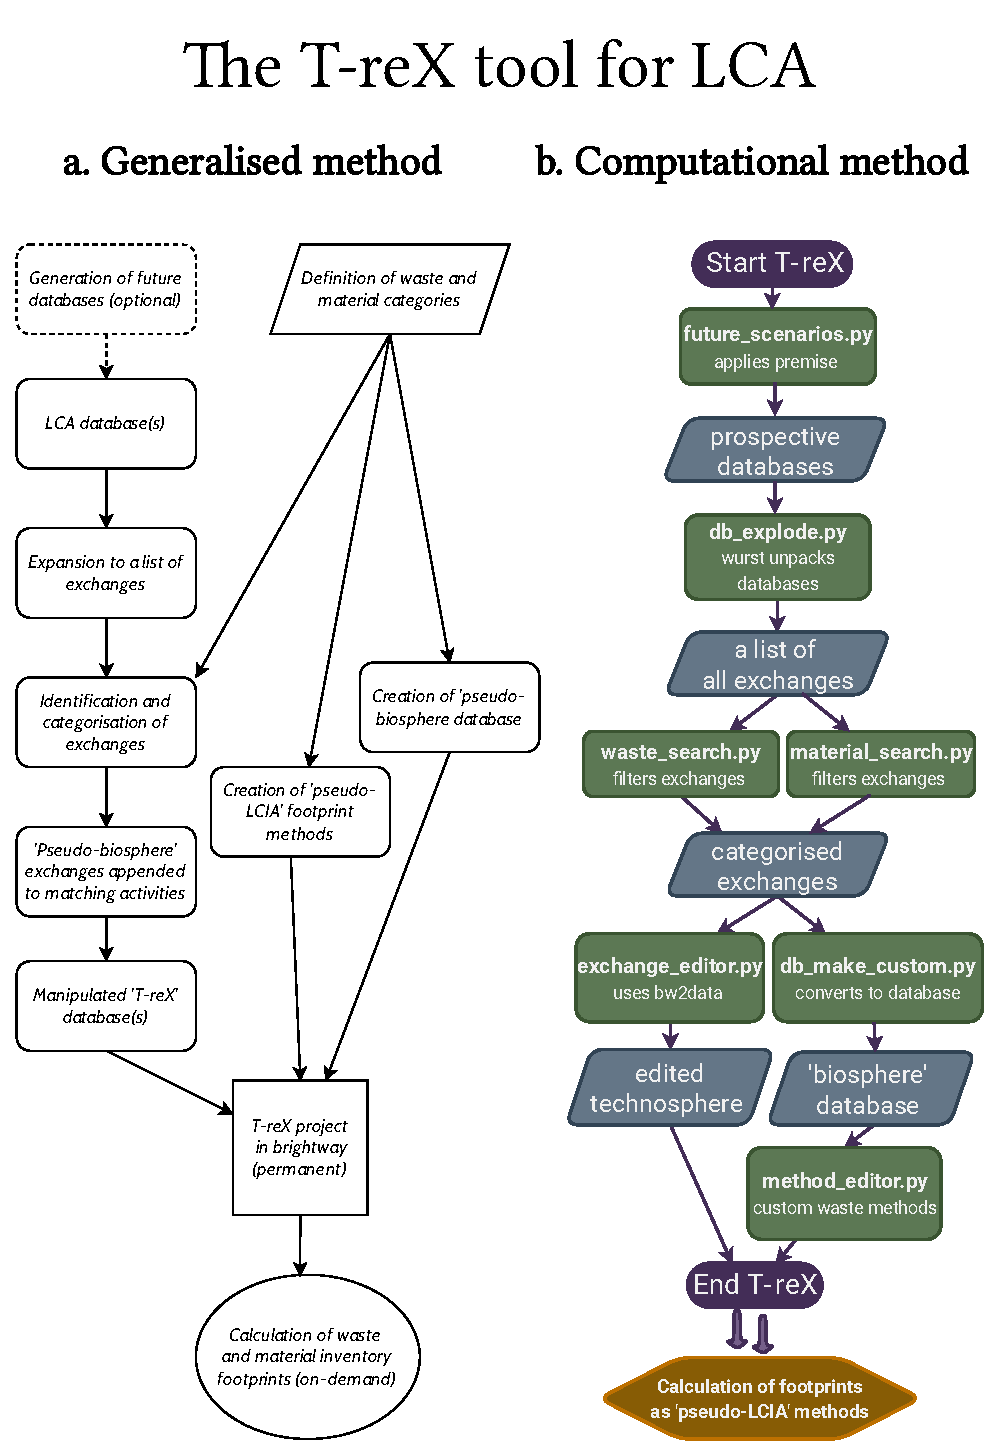
\includegraphics[height=0.8\textheight]{T-reX_flowchart-supplementary.pdf}
    \caption{The generalised (a) and computational flowcharts of T-reX. In green are the individual modules, in blue are their outputs. The final product is one or more manipulated databases with which one can calculate the material and waste inventory footprints using the `pseudo-LCIA' methods created by T-reX based on the search configuration.}\label{fig:flowchart}
\end{figure}

\clearpage

\section{Example terminal output of T-reX}

Due to its length, an example of the terminal output of T-reX is included as a separate file in the supplementary material, named `T-reX\_example\_terminal\_output.pdf'. The example output is from the execution of T-reX on the `\texttt{ecoinvent} 3.9.1' database with the IAM model `REMIND' and the RCP `PkBudg500' in the years 2065 and 2100. The example output includes the execution of the main module which in turn executes the \texttt{future\_scenarios}, \texttt{explode\_database}, \texttt{search\_waste}, \texttt{search\_material}, \texttt{make\_custom\_database}, \texttt{method\_editor}, \texttt{exchange\_editor}, and \texttt{verify\_database} modules.

Due to licensing restrictions, the manipulated \texttt{ecoinvent} databases produced by T-reX are not included in the supplementary material. However, with a licence to the \texttt{ecoinvent} database, the user can easily reproduce the results of T-reX by following the instructions in the documentation.

\clearpage


\section{Python scripts used in the case study}

The Python scripts used in the case study are included as separate \texttt{.py} files in the `case-study' folder of the supplementary material. The terminal output of the case-study calculations is included in the `case-study' folder as a \texttt{.html} file, which can be opened in an internet browser and as a plain text file.

\clearpage
\section{Complete tabulated results of the case study}

Due to their length, the complete tabulated results of the case study are included as separate files in the `case-study/data\_batteries' folder of the supplementary material. The results are presented in the form of \texttt{.csv} files. More are available in the GitHub repositories \url{https://github.com/Stew-McD/T-reX_Publication} (publication) and \url{https://github.com/Stew-McD/T-reX} (codebase).


\clearpage

\section{Complete visualisations from the case study}

Due to their size, the complete visualisations from the case study are included as separate files in the `case-study/visualisation\_batteries' folder of the supplementary material. The visualisations are presented in the form of merged \texttt{.pdf} files and separate \texttt{.svg} file. More are available in the GitHub repositories \url{https://github.com/Stew-McD/T-reX_Publication} (publication) and \url{https://github.com/Stew-McD/T-reX} (codebase).

\clearpage

\bibliographystyle{elsarticle-harv}
\bibliography{references.bib}


\end{document}